% Created by tikzDevice version 0.12.3.1 on 2021-04-13 14:29:04
% !TEX encoding = UTF-8 Unicode
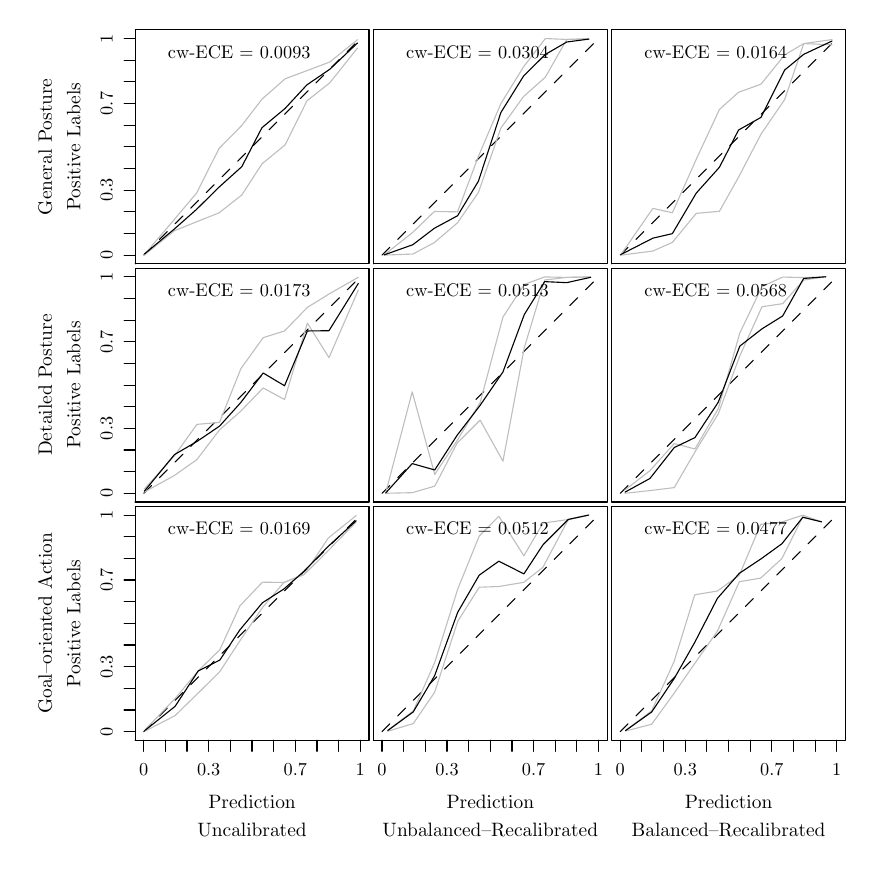
\begin{tikzpicture}[x=1pt,y=1pt]
\definecolor{fillColor}{RGB}{255,255,255}
\path[use as bounding box,fill=fillColor,fill opacity=0.00] (0,0) rectangle (296.31,296.31);
\begin{scope}
\path[clip] (  0.00,  0.00) rectangle (296.31,296.31);
\definecolor{drawColor}{RGB}{0,0,0}

\path[draw=drawColor,line width= 0.4pt,line join=round,line cap=round] ( 38.81,211.00) --
	(123.32,211.00) --
	(123.32,295.51) --
	( 38.81,295.51) --
	( 38.81,211.00);
\end{scope}
\begin{scope}
\path[clip] ( 38.81,211.00) rectangle (123.32,295.51);
\definecolor{drawColor}{RGB}{0,0,0}

\path[draw=drawColor,line width= 0.4pt,dash pattern=on 4pt off 4pt ,line join=round,line cap=round] ( 41.94,214.13) --
	(120.19,292.38);
\definecolor{drawColor}{RGB}{190,190,190}

\path[draw=drawColor,line width= 0.4pt,line join=round,line cap=round] ( 42.16,214.13) --
	( 52.97,222.91) --
	( 61.09,226.18) --
	( 69.16,229.40) --
	( 77.38,235.84) --
	( 84.65,247.09) --
	( 93.01,253.94) --
	(100.90,269.85) --
	(109.15,276.36) --
	(119.19,288.94);

\path[draw=drawColor,line width= 0.4pt,line join=round,line cap=round] ( 42.16,214.36) --
	( 52.97,226.97) --
	( 61.09,236.62) --
	( 69.16,252.67) --
	( 77.38,260.98) --
	( 84.65,270.46) --
	( 93.01,277.82) --
	(100.90,280.78) --
	(109.15,283.89) --
	(119.19,291.97);
\definecolor{drawColor}{RGB}{0,0,0}

\path[draw=drawColor,line width= 0.4pt,line join=round,line cap=round] ( 42.16,214.49) --
	( 52.97,223.52) --
	( 61.09,230.71) --
	( 69.16,238.69) --
	( 77.38,246.09) --
	( 84.65,260.16) --
	( 93.01,267.11) --
	(100.90,275.64) --
	(109.15,281.26) --
	(119.19,290.78);

\node[text=drawColor,anchor=base west,inner sep=0pt, outer sep=0pt, scale=  0.66] at ( 50.69,285.32) {cw-ECE = 0.0093};
\end{scope}
\begin{scope}
\path[clip] (  0.00,  0.00) rectangle (296.31,296.31);
\definecolor{drawColor}{RGB}{0,0,0}

\path[draw=drawColor,line width= 0.4pt,line join=round,line cap=round] ( 38.81,214.13) -- ( 38.81,292.38);

\path[draw=drawColor,line width= 0.4pt,line join=round,line cap=round] ( 38.81,214.13) -- ( 34.85,214.13);

\path[draw=drawColor,line width= 0.4pt,line join=round,line cap=round] ( 38.81,221.96) -- ( 34.85,221.96);

\path[draw=drawColor,line width= 0.4pt,line join=round,line cap=round] ( 38.81,229.78) -- ( 34.85,229.78);

\path[draw=drawColor,line width= 0.4pt,line join=round,line cap=round] ( 38.81,237.61) -- ( 34.85,237.61);

\path[draw=drawColor,line width= 0.4pt,line join=round,line cap=round] ( 38.81,245.43) -- ( 34.85,245.43);

\path[draw=drawColor,line width= 0.4pt,line join=round,line cap=round] ( 38.81,253.26) -- ( 34.85,253.26);

\path[draw=drawColor,line width= 0.4pt,line join=round,line cap=round] ( 38.81,261.08) -- ( 34.85,261.08);

\path[draw=drawColor,line width= 0.4pt,line join=round,line cap=round] ( 38.81,268.91) -- ( 34.85,268.91);

\path[draw=drawColor,line width= 0.4pt,line join=round,line cap=round] ( 38.81,276.73) -- ( 34.85,276.73);

\path[draw=drawColor,line width= 0.4pt,line join=round,line cap=round] ( 38.81,284.56) -- ( 34.85,284.56);

\path[draw=drawColor,line width= 0.4pt,line join=round,line cap=round] ( 38.81,292.38) -- ( 34.85,292.38);

\node[text=drawColor,rotate= 90.00,anchor=base,inner sep=0pt, outer sep=0pt, scale=  0.66] at ( 30.67,214.13) {0};

\node[text=drawColor,rotate= 90.00,anchor=base,inner sep=0pt, outer sep=0pt, scale=  0.66] at ( 30.67,237.61) {0.3};

\node[text=drawColor,rotate= 90.00,anchor=base,inner sep=0pt, outer sep=0pt, scale=  0.66] at ( 30.67,268.91) {0.7};

\node[text=drawColor,rotate= 90.00,anchor=base,inner sep=0pt, outer sep=0pt, scale=  0.66] at ( 30.67,292.38) {1};

\node[text=drawColor,rotate= 90.00,anchor=base,inner sep=0pt, outer sep=0pt, scale=  0.70] at ( 19.01,253.26) {Positive Labels};

\node[text=drawColor,rotate= 90.00,anchor=base,inner sep=0pt, outer sep=0pt, scale=  0.70] at (  8.71,253.26) {General Posture};
\end{scope}
\begin{scope}
\path[clip] (  0.00,  0.00) rectangle (296.31,296.31);
\definecolor{drawColor}{RGB}{0,0,0}

\path[draw=drawColor,line width= 0.4pt,line join=round,line cap=round] ( 38.81,124.90) --
	(123.32,124.90) --
	(123.32,209.42) --
	( 38.81,209.42) --
	( 38.81,124.90);
\end{scope}
\begin{scope}
\path[clip] ( 38.81,124.90) rectangle (123.32,209.42);
\definecolor{drawColor}{RGB}{0,0,0}

\path[draw=drawColor,line width= 0.4pt,dash pattern=on 4pt off 4pt ,line join=round,line cap=round] ( 41.94,128.04) --
	(120.19,206.29);
\definecolor{drawColor}{RGB}{190,190,190}

\path[draw=drawColor,line width= 0.4pt,line join=round,line cap=round] ( 42.16,128.49) --
	( 53.04,134.51) --
	( 61.15,140.24) --
	( 69.33,150.98) --
	( 77.00,157.73) --
	( 85.09,166.13) --
	( 92.82,161.93) --
	(101.07,189.56) --
	(108.87,177.07) --
	(119.48,201.49);

\path[draw=drawColor,line width= 0.4pt,line join=round,line cap=round] ( 42.16,129.62) --
	( 53.04,141.61) --
	( 61.15,152.96) --
	( 69.33,153.66) --
	( 77.00,173.03) --
	( 85.09,184.29) --
	( 92.82,186.72) --
	(101.07,195.23) --
	(108.87,200.06) --
	(119.48,206.12);
\definecolor{drawColor}{RGB}{0,0,0}

\path[draw=drawColor,line width= 0.4pt,line join=round,line cap=round] ( 42.16,128.81) --
	( 53.04,142.03) --
	( 61.15,146.77) --
	( 69.33,152.33) --
	( 77.00,160.85) --
	( 85.09,171.53) --
	( 92.82,166.91) --
	(101.07,186.71) --
	(108.87,186.81) --
	(119.48,203.88);

\node[text=drawColor,anchor=base west,inner sep=0pt, outer sep=0pt, scale=  0.66] at ( 50.69,199.23) {cw-ECE = 0.0173};
\end{scope}
\begin{scope}
\path[clip] (  0.00,  0.00) rectangle (296.31,296.31);
\definecolor{drawColor}{RGB}{0,0,0}

\path[draw=drawColor,line width= 0.4pt,line join=round,line cap=round] ( 38.81,128.04) -- ( 38.81,206.29);

\path[draw=drawColor,line width= 0.4pt,line join=round,line cap=round] ( 38.81,128.04) -- ( 34.85,128.04);

\path[draw=drawColor,line width= 0.4pt,line join=round,line cap=round] ( 38.81,135.86) -- ( 34.85,135.86);

\path[draw=drawColor,line width= 0.4pt,line join=round,line cap=round] ( 38.81,143.69) -- ( 34.85,143.69);

\path[draw=drawColor,line width= 0.4pt,line join=round,line cap=round] ( 38.81,151.51) -- ( 34.85,151.51);

\path[draw=drawColor,line width= 0.4pt,line join=round,line cap=round] ( 38.81,159.34) -- ( 34.85,159.34);

\path[draw=drawColor,line width= 0.4pt,line join=round,line cap=round] ( 38.81,167.16) -- ( 34.85,167.16);

\path[draw=drawColor,line width= 0.4pt,line join=round,line cap=round] ( 38.81,174.99) -- ( 34.85,174.99);

\path[draw=drawColor,line width= 0.4pt,line join=round,line cap=round] ( 38.81,182.81) -- ( 34.85,182.81);

\path[draw=drawColor,line width= 0.4pt,line join=round,line cap=round] ( 38.81,190.64) -- ( 34.85,190.64);

\path[draw=drawColor,line width= 0.4pt,line join=round,line cap=round] ( 38.81,198.46) -- ( 34.85,198.46);

\path[draw=drawColor,line width= 0.4pt,line join=round,line cap=round] ( 38.81,206.29) -- ( 34.85,206.29);

\node[text=drawColor,rotate= 90.00,anchor=base,inner sep=0pt, outer sep=0pt, scale=  0.66] at ( 30.67,128.04) {0};

\node[text=drawColor,rotate= 90.00,anchor=base,inner sep=0pt, outer sep=0pt, scale=  0.66] at ( 30.67,151.51) {0.3};

\node[text=drawColor,rotate= 90.00,anchor=base,inner sep=0pt, outer sep=0pt, scale=  0.66] at ( 30.67,182.81) {0.7};

\node[text=drawColor,rotate= 90.00,anchor=base,inner sep=0pt, outer sep=0pt, scale=  0.66] at ( 30.67,206.29) {1};

\node[text=drawColor,rotate= 90.00,anchor=base,inner sep=0pt, outer sep=0pt, scale=  0.70] at ( 19.01,167.16) {Positive Labels};

\node[text=drawColor,rotate= 90.00,anchor=base,inner sep=0pt, outer sep=0pt, scale=  0.70] at (  8.71,167.16) {Detailed Posture};
\end{scope}
\begin{scope}
\path[clip] (  0.00,  0.00) rectangle (296.31,296.31);
\definecolor{drawColor}{RGB}{0,0,0}

\path[draw=drawColor,line width= 0.4pt,line join=round,line cap=round] ( 38.81, 38.81) --
	(123.32, 38.81) --
	(123.32,123.32) --
	( 38.81,123.32) --
	( 38.81, 38.81);
\end{scope}
\begin{scope}
\path[clip] ( 38.81, 38.81) rectangle (123.32,123.32);
\definecolor{drawColor}{RGB}{0,0,0}

\path[draw=drawColor,line width= 0.4pt,dash pattern=on 4pt off 4pt ,line join=round,line cap=round] ( 41.94, 41.94) --
	(120.19,120.19);
\definecolor{drawColor}{RGB}{190,190,190}

\path[draw=drawColor,line width= 0.4pt,line join=round,line cap=round] ( 42.51, 42.18) --
	( 53.26, 47.71) --
	( 61.63, 55.90) --
	( 69.43, 63.63) --
	( 76.68, 74.74) --
	( 84.84, 86.79) --
	( 92.56, 95.83) --
	( 99.87, 98.66) --
	(108.61,107.34) --
	(118.70,117.69);

\path[draw=drawColor,line width= 0.4pt,line join=round,line cap=round] ( 42.51, 42.69) --
	( 53.26, 53.88) --
	( 61.63, 63.90) --
	( 69.43, 71.52) --
	( 76.68, 87.39) --
	( 84.84, 95.94) --
	( 92.56, 95.83) --
	( 99.87, 98.75) --
	(108.61,111.89) --
	(118.70,119.99);
\definecolor{drawColor}{RGB}{0,0,0}

\path[draw=drawColor,line width= 0.4pt,line join=round,line cap=round] ( 42.51, 42.47) --
	( 53.26, 51.06) --
	( 61.63, 63.86) --
	( 69.43, 67.79) --
	( 76.68, 78.70) --
	( 84.84, 88.51) --
	( 92.56, 93.45) --
	( 99.87, 99.89) --
	(108.61,108.89) --
	(118.70,118.12);

\node[text=drawColor,anchor=base west,inner sep=0pt, outer sep=0pt, scale=  0.66] at ( 50.69,113.13) {cw-ECE = 0.0169};
\end{scope}
\begin{scope}
\path[clip] (  0.00,  0.00) rectangle (296.31,296.31);
\definecolor{drawColor}{RGB}{0,0,0}

\path[draw=drawColor,line width= 0.4pt,line join=round,line cap=round] ( 41.94, 38.81) -- (120.19, 38.81);

\path[draw=drawColor,line width= 0.4pt,line join=round,line cap=round] ( 41.94, 38.81) -- ( 41.94, 34.85);

\path[draw=drawColor,line width= 0.4pt,line join=round,line cap=round] ( 49.76, 38.81) -- ( 49.76, 34.85);

\path[draw=drawColor,line width= 0.4pt,line join=round,line cap=round] ( 57.59, 38.81) -- ( 57.59, 34.85);

\path[draw=drawColor,line width= 0.4pt,line join=round,line cap=round] ( 65.41, 38.81) -- ( 65.41, 34.85);

\path[draw=drawColor,line width= 0.4pt,line join=round,line cap=round] ( 73.24, 38.81) -- ( 73.24, 34.85);

\path[draw=drawColor,line width= 0.4pt,line join=round,line cap=round] ( 81.06, 38.81) -- ( 81.06, 34.85);

\path[draw=drawColor,line width= 0.4pt,line join=round,line cap=round] ( 88.89, 38.81) -- ( 88.89, 34.85);

\path[draw=drawColor,line width= 0.4pt,line join=round,line cap=round] ( 96.72, 38.81) -- ( 96.72, 34.85);

\path[draw=drawColor,line width= 0.4pt,line join=round,line cap=round] (104.54, 38.81) -- (104.54, 34.85);

\path[draw=drawColor,line width= 0.4pt,line join=round,line cap=round] (112.37, 38.81) -- (112.37, 34.85);

\path[draw=drawColor,line width= 0.4pt,line join=round,line cap=round] (120.19, 38.81) -- (120.19, 34.85);

\node[text=drawColor,anchor=base,inner sep=0pt, outer sep=0pt, scale=  0.66] at ( 41.94, 25.92) {0};

\node[text=drawColor,anchor=base,inner sep=0pt, outer sep=0pt, scale=  0.66] at ( 65.41, 25.92) {0.3};

\node[text=drawColor,anchor=base,inner sep=0pt, outer sep=0pt, scale=  0.66] at ( 96.72, 25.92) {0.7};

\node[text=drawColor,anchor=base,inner sep=0pt, outer sep=0pt, scale=  0.66] at (120.19, 25.92) {1};

\node[text=drawColor,anchor=base,inner sep=0pt, outer sep=0pt, scale=  0.70] at ( 81.06, 14.26) {Prediction};

\node[text=drawColor,anchor=base,inner sep=0pt, outer sep=0pt, scale=  0.70] at ( 81.06,  3.96) {Uncalibrated};

\path[draw=drawColor,line width= 0.4pt,line join=round,line cap=round] ( 38.81, 41.94) -- ( 38.81,120.19);

\path[draw=drawColor,line width= 0.4pt,line join=round,line cap=round] ( 38.81, 41.94) -- ( 34.85, 41.94);

\path[draw=drawColor,line width= 0.4pt,line join=round,line cap=round] ( 38.81, 49.76) -- ( 34.85, 49.76);

\path[draw=drawColor,line width= 0.4pt,line join=round,line cap=round] ( 38.81, 57.59) -- ( 34.85, 57.59);

\path[draw=drawColor,line width= 0.4pt,line join=round,line cap=round] ( 38.81, 65.41) -- ( 34.85, 65.41);

\path[draw=drawColor,line width= 0.4pt,line join=round,line cap=round] ( 38.81, 73.24) -- ( 34.85, 73.24);

\path[draw=drawColor,line width= 0.4pt,line join=round,line cap=round] ( 38.81, 81.06) -- ( 34.85, 81.06);

\path[draw=drawColor,line width= 0.4pt,line join=round,line cap=round] ( 38.81, 88.89) -- ( 34.85, 88.89);

\path[draw=drawColor,line width= 0.4pt,line join=round,line cap=round] ( 38.81, 96.72) -- ( 34.85, 96.72);

\path[draw=drawColor,line width= 0.4pt,line join=round,line cap=round] ( 38.81,104.54) -- ( 34.85,104.54);

\path[draw=drawColor,line width= 0.4pt,line join=round,line cap=round] ( 38.81,112.37) -- ( 34.85,112.37);

\path[draw=drawColor,line width= 0.4pt,line join=round,line cap=round] ( 38.81,120.19) -- ( 34.85,120.19);

\node[text=drawColor,rotate= 90.00,anchor=base,inner sep=0pt, outer sep=0pt, scale=  0.66] at ( 30.67, 41.94) {0};

\node[text=drawColor,rotate= 90.00,anchor=base,inner sep=0pt, outer sep=0pt, scale=  0.66] at ( 30.67, 65.41) {0.3};

\node[text=drawColor,rotate= 90.00,anchor=base,inner sep=0pt, outer sep=0pt, scale=  0.66] at ( 30.67, 96.72) {0.7};

\node[text=drawColor,rotate= 90.00,anchor=base,inner sep=0pt, outer sep=0pt, scale=  0.66] at ( 30.67,120.19) {1};

\node[text=drawColor,rotate= 90.00,anchor=base,inner sep=0pt, outer sep=0pt, scale=  0.70] at ( 19.01, 81.06) {Positive Labels};

\node[text=drawColor,rotate= 90.00,anchor=base,inner sep=0pt, outer sep=0pt, scale=  0.70] at (  8.71, 81.06) {Goal--oriented Action};
\end{scope}
\begin{scope}
\path[clip] (  0.00,  0.00) rectangle (296.31,296.31);
\definecolor{drawColor}{RGB}{0,0,0}

\path[draw=drawColor,line width= 0.4pt,line join=round,line cap=round] (124.90,211.00) --
	(209.42,211.00) --
	(209.42,295.51) --
	(124.90,295.51) --
	(124.90,211.00);
\end{scope}
\begin{scope}
\path[clip] (124.90,211.00) rectangle (209.42,295.51);
\definecolor{drawColor}{RGB}{0,0,0}

\path[draw=drawColor,line width= 0.4pt,dash pattern=on 4pt off 4pt ,line join=round,line cap=round] (128.04,214.13) --
	(206.29,292.38);
\definecolor{drawColor}{RGB}{190,190,190}

\path[draw=drawColor,line width= 0.4pt,line join=round,line cap=round] (128.83,214.13) --
	(139.17,214.50) --
	(146.95,218.65) --
	(155.34,225.81) --
	(162.89,236.80) --
	(170.99,260.03) --
	(179.21,271.44) --
	(187.06,278.43) --
	(194.81,292.05) --
	(202.80,292.09);

\path[draw=drawColor,line width= 0.4pt,line join=round,line cap=round] (128.83,214.18) --
	(139.17,222.36) --
	(146.95,229.88) --
	(155.34,229.76) --
	(162.89,249.85) --
	(170.99,268.88) --
	(179.21,282.21) --
	(187.06,292.38) --
	(194.81,292.05) --
	(202.80,292.38);
\definecolor{drawColor}{RGB}{0,0,0}

\path[draw=drawColor,line width= 0.4pt,line join=round,line cap=round] (128.83,214.20) --
	(139.17,217.88) --
	(146.95,223.82) --
	(155.34,228.35) --
	(162.89,240.86) --
	(170.99,265.65) --
	(179.21,278.85) --
	(187.06,286.64) --
	(194.81,291.13) --
	(202.80,292.18);

\node[text=drawColor,anchor=base west,inner sep=0pt, outer sep=0pt, scale=  0.66] at (136.78,285.32) {cw-ECE = 0.0304};
\end{scope}
\begin{scope}
\path[clip] (  0.00,  0.00) rectangle (296.31,296.31);
\definecolor{drawColor}{RGB}{0,0,0}

\path[draw=drawColor,line width= 0.4pt,line join=round,line cap=round] (124.90,124.90) --
	(209.42,124.90) --
	(209.42,209.42) --
	(124.90,209.42) --
	(124.90,124.90);
\end{scope}
\begin{scope}
\path[clip] (124.90,124.90) rectangle (209.42,209.42);
\definecolor{drawColor}{RGB}{0,0,0}

\path[draw=drawColor,line width= 0.4pt,dash pattern=on 4pt off 4pt ,line join=round,line cap=round] (128.04,128.04) --
	(206.29,206.29);
\definecolor{drawColor}{RGB}{190,190,190}

\path[draw=drawColor,line width= 0.4pt,line join=round,line cap=round] (129.40,128.06) --
	(138.95,128.28) --
	(147.09,130.63) --
	(155.19,146.21) --
	(163.49,154.49) --
	(171.74,139.65) --
	(179.45,180.66) --
	(186.82,205.13) --
	(194.77,206.06) --
	(203.44,206.26);

\path[draw=drawColor,line width= 0.4pt,line join=round,line cap=round] (129.40,128.30) --
	(138.95,164.71) --
	(147.09,134.88) --
	(155.19,147.11) --
	(163.49,160.82) --
	(171.74,191.75) --
	(179.45,203.53) --
	(186.82,206.24) --
	(194.77,206.06) --
	(203.44,206.26);
\definecolor{drawColor}{RGB}{0,0,0}

\path[draw=drawColor,line width= 0.4pt,line join=round,line cap=round] (129.40,128.20) --
	(138.95,138.79) --
	(147.09,136.48) --
	(155.19,149.03) --
	(163.49,159.83) --
	(171.74,171.90) --
	(179.45,192.64) --
	(186.82,204.54) --
	(194.77,204.17) --
	(203.44,206.10);

\node[text=drawColor,anchor=base west,inner sep=0pt, outer sep=0pt, scale=  0.66] at (136.78,199.23) {cw-ECE = 0.0513};
\end{scope}
\begin{scope}
\path[clip] (  0.00,  0.00) rectangle (296.31,296.31);
\definecolor{drawColor}{RGB}{0,0,0}

\path[draw=drawColor,line width= 0.4pt,line join=round,line cap=round] (124.90, 38.81) --
	(209.42, 38.81) --
	(209.42,123.32) --
	(124.90,123.32) --
	(124.90, 38.81);
\end{scope}
\begin{scope}
\path[clip] (124.90, 38.81) rectangle (209.42,123.32);
\definecolor{drawColor}{RGB}{0,0,0}

\path[draw=drawColor,line width= 0.4pt,dash pattern=on 4pt off 4pt ,line join=round,line cap=round] (128.04, 41.94) --
	(206.29,120.19);
\definecolor{drawColor}{RGB}{190,190,190}

\path[draw=drawColor,line width= 0.4pt,line join=round,line cap=round] (130.11, 42.08) --
	(139.33, 44.84) --
	(147.05, 56.15) --
	(155.39, 81.77) --
	(163.16, 94.12) --
	(170.25, 94.37) --
	(179.31, 95.90) --
	(186.18,101.31) --
	(195.35,118.59) --
	(202.73,120.19);

\path[draw=drawColor,line width= 0.4pt,line join=round,line cap=round] (130.11, 42.42) --
	(139.33, 49.38) --
	(147.05, 66.83) --
	(155.39, 93.42) --
	(163.16,112.61) --
	(170.25,119.72) --
	(179.31,105.48) --
	(186.18,117.26) --
	(195.35,118.59) --
	(202.73,120.19);
\definecolor{drawColor}{RGB}{0,0,0}

\path[draw=drawColor,line width= 0.4pt,line join=round,line cap=round] (130.11, 42.33) --
	(139.33, 49.07) --
	(147.05, 62.13) --
	(155.39, 85.06) --
	(163.16, 98.47) --
	(170.25,103.52) --
	(179.31, 98.94) --
	(186.18,109.42) --
	(195.35,118.61) --
	(202.73,120.19);

\node[text=drawColor,anchor=base west,inner sep=0pt, outer sep=0pt, scale=  0.66] at (136.78,113.13) {cw-ECE = 0.0512};
\end{scope}
\begin{scope}
\path[clip] (  0.00,  0.00) rectangle (296.31,296.31);
\definecolor{drawColor}{RGB}{0,0,0}

\path[draw=drawColor,line width= 0.4pt,line join=round,line cap=round] (128.04, 38.81) -- (206.29, 38.81);

\path[draw=drawColor,line width= 0.4pt,line join=round,line cap=round] (128.04, 38.81) -- (128.04, 34.85);

\path[draw=drawColor,line width= 0.4pt,line join=round,line cap=round] (135.86, 38.81) -- (135.86, 34.85);

\path[draw=drawColor,line width= 0.4pt,line join=round,line cap=round] (143.69, 38.81) -- (143.69, 34.85);

\path[draw=drawColor,line width= 0.4pt,line join=round,line cap=round] (151.51, 38.81) -- (151.51, 34.85);

\path[draw=drawColor,line width= 0.4pt,line join=round,line cap=round] (159.34, 38.81) -- (159.34, 34.85);

\path[draw=drawColor,line width= 0.4pt,line join=round,line cap=round] (167.16, 38.81) -- (167.16, 34.85);

\path[draw=drawColor,line width= 0.4pt,line join=round,line cap=round] (174.99, 38.81) -- (174.99, 34.85);

\path[draw=drawColor,line width= 0.4pt,line join=round,line cap=round] (182.81, 38.81) -- (182.81, 34.85);

\path[draw=drawColor,line width= 0.4pt,line join=round,line cap=round] (190.64, 38.81) -- (190.64, 34.85);

\path[draw=drawColor,line width= 0.4pt,line join=round,line cap=round] (198.46, 38.81) -- (198.46, 34.85);

\path[draw=drawColor,line width= 0.4pt,line join=round,line cap=round] (206.29, 38.81) -- (206.29, 34.85);

\node[text=drawColor,anchor=base,inner sep=0pt, outer sep=0pt, scale=  0.66] at (128.04, 25.92) {0};

\node[text=drawColor,anchor=base,inner sep=0pt, outer sep=0pt, scale=  0.66] at (151.51, 25.92) {0.3};

\node[text=drawColor,anchor=base,inner sep=0pt, outer sep=0pt, scale=  0.66] at (182.81, 25.92) {0.7};

\node[text=drawColor,anchor=base,inner sep=0pt, outer sep=0pt, scale=  0.66] at (206.29, 25.92) {1};

\node[text=drawColor,anchor=base,inner sep=0pt, outer sep=0pt, scale=  0.70] at (167.16, 14.26) {Prediction};

\node[text=drawColor,anchor=base,inner sep=0pt, outer sep=0pt, scale=  0.70] at (167.16,  3.96) {Unbalanced--Recalibrated};
\end{scope}
\begin{scope}
\path[clip] (  0.00,  0.00) rectangle (296.31,296.31);
\definecolor{drawColor}{RGB}{0,0,0}

\path[draw=drawColor,line width= 0.4pt,line join=round,line cap=round] (211.00,211.00) --
	(295.51,211.00) --
	(295.51,295.51) --
	(211.00,295.51) --
	(211.00,211.00);
\end{scope}
\begin{scope}
\path[clip] (211.00,211.00) rectangle (295.51,295.51);
\definecolor{drawColor}{RGB}{0,0,0}

\path[draw=drawColor,line width= 0.4pt,dash pattern=on 4pt off 4pt ,line join=round,line cap=round] (214.13,214.13) --
	(292.38,292.38);
\definecolor{drawColor}{RGB}{190,190,190}

\path[draw=drawColor,line width= 0.4pt,line join=round,line cap=round] (214.52,214.13) --
	(225.93,215.60) --
	(232.95,218.71) --
	(241.60,229.20) --
	(249.96,229.96) --
	(256.87,242.27) --
	(264.98,257.82) --
	(273.52,270.31) --
	(280.43,290.56) --
	(290.66,290.11);

\path[draw=drawColor,line width= 0.4pt,line join=round,line cap=round] (214.52,214.54) --
	(225.93,231.01) --
	(232.95,229.42) --
	(241.60,248.77) --
	(249.96,266.75) --
	(256.87,272.96) --
	(264.98,275.88) --
	(273.52,286.46) --
	(280.43,290.56) --
	(290.66,292.01);
\definecolor{drawColor}{RGB}{0,0,0}

\path[draw=drawColor,line width= 0.4pt,line join=round,line cap=round] (214.52,214.42) --
	(225.93,220.25) --
	(232.95,221.88) --
	(241.60,236.54) --
	(249.96,245.87) --
	(256.87,259.32) --
	(264.98,263.89) --
	(273.52,280.99) --
	(280.43,286.68) --
	(290.66,291.48);

\node[text=drawColor,anchor=base west,inner sep=0pt, outer sep=0pt, scale=  0.66] at (222.88,285.32) {cw-ECE = 0.0164};
\end{scope}
\begin{scope}
\path[clip] (  0.00,  0.00) rectangle (296.31,296.31);
\definecolor{drawColor}{RGB}{0,0,0}

\path[draw=drawColor,line width= 0.4pt,line join=round,line cap=round] (211.00,124.90) --
	(295.51,124.90) --
	(295.51,209.42) --
	(211.00,209.42) --
	(211.00,124.90);
\end{scope}
\begin{scope}
\path[clip] (211.00,124.90) rectangle (295.51,209.42);
\definecolor{drawColor}{RGB}{0,0,0}

\path[draw=drawColor,line width= 0.4pt,dash pattern=on 4pt off 4pt ,line join=round,line cap=round] (214.13,128.04) --
	(292.38,206.29);
\definecolor{drawColor}{RGB}{190,190,190}

\path[draw=drawColor,line width= 0.4pt,line join=round,line cap=round] (215.85,128.06) --
	(224.84,129.04) --
	(233.64,130.11) --
	(241.12,143.01) --
	(249.54,156.76) --
	(257.34,177.75) --
	(265.35,195.46) --
	(272.81,196.58) --
	(280.40,205.11) --
	(288.39,206.29);

\path[draw=drawColor,line width= 0.4pt,line join=round,line cap=round] (215.85,129.28) --
	(224.84,136.22) --
	(233.64,146.02) --
	(241.12,144.07) --
	(249.54,158.59) --
	(257.34,185.98) --
	(265.35,202.74) --
	(272.81,206.18) --
	(280.40,206.01) --
	(288.39,206.29);
\definecolor{drawColor}{RGB}{0,0,0}

\path[draw=drawColor,line width= 0.4pt,line join=round,line cap=round] (215.85,128.48) --
	(224.84,133.40) --
	(233.64,144.58) --
	(241.12,148.19) --
	(249.54,160.97) --
	(257.34,181.25) --
	(265.35,187.49) --
	(272.81,192.13) --
	(280.40,205.69) --
	(288.39,206.29);

\node[text=drawColor,anchor=base west,inner sep=0pt, outer sep=0pt, scale=  0.66] at (222.88,199.23) {cw-ECE = 0.0568};
\end{scope}
\begin{scope}
\path[clip] (  0.00,  0.00) rectangle (296.31,296.31);
\definecolor{drawColor}{RGB}{0,0,0}

\path[draw=drawColor,line width= 0.4pt,line join=round,line cap=round] (211.00, 38.81) --
	(295.51, 38.81) --
	(295.51,123.32) --
	(211.00,123.32) --
	(211.00, 38.81);
\end{scope}
\begin{scope}
\path[clip] (211.00, 38.81) rectangle (295.51,123.32);
\definecolor{drawColor}{RGB}{0,0,0}

\path[draw=drawColor,line width= 0.4pt,dash pattern=on 4pt off 4pt ,line join=round,line cap=round] (214.13, 41.94) --
	(292.38,120.19);
\definecolor{drawColor}{RGB}{190,190,190}

\path[draw=drawColor,line width= 0.4pt,line join=round,line cap=round] (216.06, 42.14) --
	(225.48, 44.62) --
	(233.58, 55.79) --
	(241.04, 66.56) --
	(249.22, 78.22) --
	(257.16, 96.11) --
	(264.88, 97.41) --
	(272.55,104.50) --
	(280.09,119.56) --
	(286.87,117.74);

\path[draw=drawColor,line width= 0.4pt,line join=round,line cap=round] (216.06, 42.39) --
	(225.48, 49.44) --
	(233.58, 67.26) --
	(241.04, 91.38) --
	(249.22, 92.75) --
	(257.16, 98.48) --
	(264.88,116.84) --
	(272.55,117.68) --
	(280.09,120.14) --
	(286.87,117.74);
\definecolor{drawColor}{RGB}{0,0,0}

\path[draw=drawColor,line width= 0.4pt,line join=round,line cap=round] (216.06, 42.32) --
	(225.48, 49.04) --
	(233.58, 61.06) --
	(241.04, 74.17) --
	(249.22, 90.07) --
	(257.16, 99.15) --
	(264.88,104.28) --
	(272.55,109.84) --
	(280.09,119.39) --
	(286.87,117.74);

\node[text=drawColor,anchor=base west,inner sep=0pt, outer sep=0pt, scale=  0.66] at (222.88,113.13) {cw-ECE = 0.0477};
\end{scope}
\begin{scope}
\path[clip] (  0.00,  0.00) rectangle (296.31,296.31);
\definecolor{drawColor}{RGB}{0,0,0}

\path[draw=drawColor,line width= 0.4pt,line join=round,line cap=round] (214.13, 38.81) -- (292.38, 38.81);

\path[draw=drawColor,line width= 0.4pt,line join=round,line cap=round] (214.13, 38.81) -- (214.13, 34.85);

\path[draw=drawColor,line width= 0.4pt,line join=round,line cap=round] (221.96, 38.81) -- (221.96, 34.85);

\path[draw=drawColor,line width= 0.4pt,line join=round,line cap=round] (229.78, 38.81) -- (229.78, 34.85);

\path[draw=drawColor,line width= 0.4pt,line join=round,line cap=round] (237.61, 38.81) -- (237.61, 34.85);

\path[draw=drawColor,line width= 0.4pt,line join=round,line cap=round] (245.43, 38.81) -- (245.43, 34.85);

\path[draw=drawColor,line width= 0.4pt,line join=round,line cap=round] (253.26, 38.81) -- (253.26, 34.85);

\path[draw=drawColor,line width= 0.4pt,line join=round,line cap=round] (261.08, 38.81) -- (261.08, 34.85);

\path[draw=drawColor,line width= 0.4pt,line join=round,line cap=round] (268.91, 38.81) -- (268.91, 34.85);

\path[draw=drawColor,line width= 0.4pt,line join=round,line cap=round] (276.73, 38.81) -- (276.73, 34.85);

\path[draw=drawColor,line width= 0.4pt,line join=round,line cap=round] (284.56, 38.81) -- (284.56, 34.85);

\path[draw=drawColor,line width= 0.4pt,line join=round,line cap=round] (292.38, 38.81) -- (292.38, 34.85);

\node[text=drawColor,anchor=base,inner sep=0pt, outer sep=0pt, scale=  0.66] at (214.13, 25.92) {0};

\node[text=drawColor,anchor=base,inner sep=0pt, outer sep=0pt, scale=  0.66] at (237.61, 25.92) {0.3};

\node[text=drawColor,anchor=base,inner sep=0pt, outer sep=0pt, scale=  0.66] at (268.91, 25.92) {0.7};

\node[text=drawColor,anchor=base,inner sep=0pt, outer sep=0pt, scale=  0.66] at (292.38, 25.92) {1};

\node[text=drawColor,anchor=base,inner sep=0pt, outer sep=0pt, scale=  0.70] at (253.26, 14.26) {Prediction};

\node[text=drawColor,anchor=base,inner sep=0pt, outer sep=0pt, scale=  0.70] at (253.26,  3.96) {Balanced--Recalibrated};
\end{scope}
\end{tikzpicture}
